\documentclass[tikz,convert={outfile=\jobname.svg}]{standalone}
\usepackage{amssymb}
\usetikzlibrary{automata, arrows.meta, positioning}
\begin{document} 
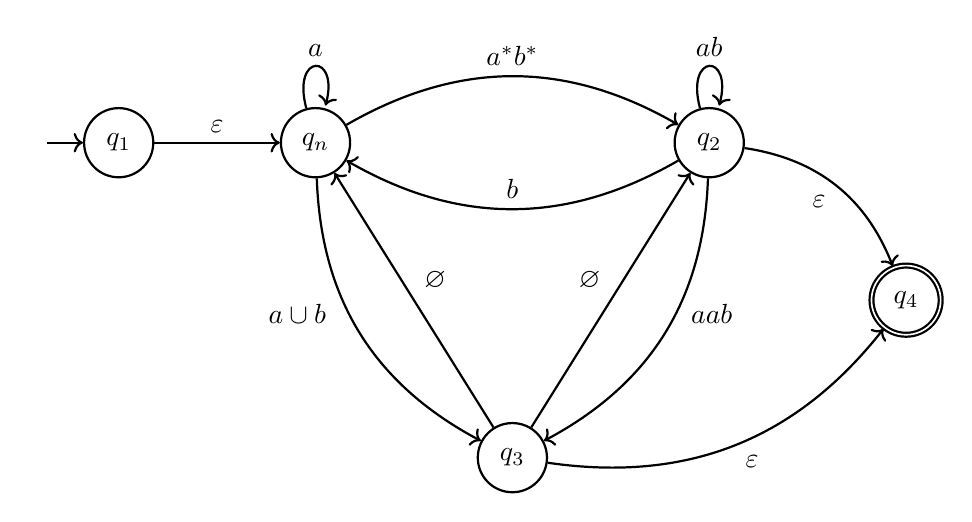
\begin{tikzpicture}[
    thick,
    node distance={25mm},
    auto
]

\node[state, initial, initial text = {}] (q1) {$q_1$}; 
\node[state] (qn) [right of=q1] {$q_n$}; 
\node[state] (q3) [below=4cm, right of=qn] {$q_3$};
\node[state] (q2) [above=4cm, right of=q3] {$q_2$}; 
\node[state, accepting] (q4) [below=2cm, right of=q2] {$q_4$};

\path[->]
    (q1) edge node {$\varepsilon$} (qn)
    (qn) edge [loop above]  node {$a$} (qn)
    (qn) edge [bend left]  node {$a^{*}b^{*}$} (q2)
    (qn) edge [bend right]  node [swap, left=0.8cm, above] {$a\cup b$} (q3)
    (q2) edge [loop above]  node {$ab$} (q2)
    (q2) edge [bend left]  node [swap] {$b$} (qn)
    (q2) edge [bend left]  node [right=0.6cm, above] {$aab$} (q3)
    (q3) edge []  node [] {$\varnothing$} (q2)
    (q3) edge []  node [swap] {$\varnothing$} (qn)
    (q2) edge [bend left]  node [swap] {$\varepsilon$} (q4)
    (q3) edge [bend right]  node [swap] {$\varepsilon$} (q4)
    ;

\end{tikzpicture} 
\end{document}
